% !TeX encoding = UTF-8
% !TeX program = lualatex
% !TeX spellcheck = en_US


\documentclass[presentation,english,aspectratio=169]{beamer}
% !TeX encoding = UTF-8
% !TeX spellcheck = en_US
% !TeX root = LoopOptTutorial.tex

% Remove the annoying symbols no one uses anyway.
\beamertemplatenavigationsymbolsempty

% Most of these were autogenerated by org export to beamer.tex file
% I don't know if they are all necessary, but I don't think there is any harm in
% including them.
\usepackage[utf8]{luainputenc}
%\usepackage[T1]{fontenc} %MK: LuaLaTeX only properly supports unicode fonts ("TU")

\usepackage{graphicx}
%\usepackage{grffile} %MK: https://github.com/ho-tex/oberdiek/issues/73
\usepackage{longtable}
\usepackage{wrapfig}
\usepackage{rotating}
\usepackage[normalem]{ulem}
\usepackage{amsmath}
\usepackage{textcomp}
\usepackage{amssymb}
\usepackage{capt-of}
\usepackage{hyperref}
\usepackage{comment}
\usetheme{default}

% I'm not sure what exactly this is for
% It is copied from a template provided by Till Tantau
% <tantau@users.sourceforge.net>
%\usepackage[english]{babel} %MK: for LuaLaTeX, use polyglossia (if needed)

% It is copied from a template provided by Till Tantau
% <tantau@users.sourceforge.net>
% I'm not sure what exactly this is for
%\usepackage{times} %MK: Not available for unicode fonts (it's a Type-1 font, obsolete and its maintainer is dead); use \uspackage{fontspec} to customize font.

\usepackage{listings}
\usepackage{xcolor}
\usepackage{minibox}
\usepackage{tikz}
\usetikzlibrary{decorations.text}
\usetikzlibrary{shapes.arrows}
\usetikzlibrary{arrows.meta}
\usetikzlibrary{bending}
\usetikzlibrary{shadows}
\usetikzlibrary{fit}
\usetikzlibrary{graphs}
\usetikzlibrary{graphdrawing}
\usetikzlibrary{matrix}
\usetikzlibrary{positioning}
\usegdlibrary{layered}

\pgfdeclarelayer{backbackbackground}
\pgfdeclarelayer{backbackground}
\pgfdeclarelayer{background}
\pgfdeclarelayer{foreground}
\pgfdeclarelayer{foreforeground}
\pgfsetlayers{backbackbackground,backbackground,background,main,foreground,foreforeground}
\tikzset{>={Stealth[round,flex,length=5pt 4.5 0.8]}} % Standard latex arrow tips are way too small
\tikzset{tight/.style={minimum width=0pt,minimum height=0pt,inner sep=0pt,outer sep=0pt}}
\usepackage{aobs-tikz}

\usepackage{minted}
\newmintinline{c}{style=bw}
\newmintinline{cpp}{style=bw}
\newmintinline{llvm}{}
\newmintinline{text}{style=bw}
\usemintedstyle{borland}

\lstset{
  basicstyle=\ttfamily,
  columns=fullflexible,
  breaklines=true,
  postbreak=\raisebox{0ex}[0ex][0ex]{\color{red}$\hookrightarrow$\space}
}

% Use this to adjust text for overlays
% If set to transparent, then text is overlays is visible, but greyed out.
% If not set, then the text in overlays is not visible at all (i.e., invisible).
\setbeamercovered{transparent}

\usecolortheme{}
\usefonttheme{}
\useinnertheme{}
\useoutertheme{}

\setbeamertemplate{blocks}[rounded][shadow=true]
\setbeamercolor{block title}{bg=teal,fg=white}
\setbeamercolor{block body}{bg=teal!10}

% Delete this, if you do not want the table of contents to pop up at
% the beginning of each subsection:
%% \AtBeginSubsection[]
%% {
%%   \begin{frame}<beamer>{Outline}
%%     \tableofcontents[currentsection,currentsubsection]
%%   \end{frame}
%% }


% If you wish to uncover everything in a step-wise fashion, uncomment
% the following command:

%\beamerdefaultoverlayspecification{<+->}



\makeatletter
% pgf 'file' shape
\def\myfoldheight{0.5}
\def\myshapepath{
	\pgfextract@process\northwest{
		\southwest\pgf@xa=\pgf@x
		\northeast
		\pgf@x=\pgf@xa
	}

	\pgfextract@process\southeast{
		\southwest\pgf@ya=\pgf@y
		\northeast
		\pgf@y=\pgf@ya
	}

	\pgfextract@process\northfold{
		\pgfpointdiff{\southwest}{\northeast}
		\northeast
		\advance\pgf@x-\myfoldheight\pgf@y
	}

	\pgfextract@process\eastfold{
		\pgfpointdiff{\southwest}{\northeast}
		\northeast
		\advance\pgf@y-\myfoldheight\pgf@y
	}

	\pgfextract@process\fold{
		\northfold\pgf@xa=\pgf@x
		\eastfold
		\pgf@x=\pgf@xa
	}

	\pgfpathmoveto{\southwest}
	\pgfpathlineto{\northwest}
	\pgfpathlineto{\northfold}
	\pgfpathlineto{\eastfold}
	\pgfpathlineto{\southeast}
	\pgfpathclose
}

% compute an intersection point between a line and \myshapepath
% NOTE: Breaks inside \graph[layered layout]
\def\myshapeanchorborder#1#2{
	% #1 = point inside the shape
	% #2 = direction
	\pgftransformreset % without this, the intersection commands yield strange results
	\pgf@relevantforpicturesizefalse % don't include drawings in bounding box
	\pgfintersectionofpaths{
		\myshapepath
		%\pgfgetpath\temppath\pgfusepath{stroke}\pgfsetpath\temppath % draw path for debugging
	}{
		\pgfpathmoveto{
			\pgfpointadd{
				\pgfpointdiff{\southwest}{\northeast}\pgf@xc=\pgf@x \advance\pgf@xc by \pgf@y % calculate a distance that is guaranteed to be outside the shape
				\pgfpointscale{
					\pgf@xc
				}{
					\pgfpointnormalised{
						#2
					}
				}
			} {
				#1
			}
		}
		\pgfpathlineto{#1}
		%\pgfgetpath\temppath\pgfusepath{stroke}\pgfsetpath\temppath % draw path for debugging
	}
	\pgfpointintersectionsolution{1}
}
\def\myshapeanchorcenter{
	\pgfpointscale{.5}{\pgfpointadd{\southwest}{\northeast}}
}

% we could probably re-use some existing \dimen, but better be careful
\newdimen\myshapedimenx
\newdimen\myshapedimeny

\pgfdeclareshape{file}{
	% some stuff, we can inherit from the rectangle shape
	\inheritsavedanchors[from=rectangle]
	\inheritanchor[from=rectangle]{center}
	\inheritanchor[from=rectangle]{mid}
	\inheritanchor[from=rectangle]{base}

	% calculate these anchors so they lie on a coorinate line with .center
	\inheritanchor[from=rectangle]{west}
	\inheritanchor[from=rectangle]{east}
	\inheritanchor[from=rectangle]{north}
	\inheritanchor[from=rectangle]{south}

	% calculate these anchors so they lie on a line through .center and the corresponding anchor of the underlying rectangle
	\inheritanchor[from=rectangle]{south west}
	\inheritanchor[from=rectangle]{south east}
	\inheritanchor[from=rectangle]{north west}
	%    \inheritanchor[from=rectangle]{north east}

	% somewhat more special anchors. The coordinate calculations were taken from the rectangle node
	\inheritanchor[from=rectangle]{mid west}
	\inheritanchor[from=rectangle]{mid east}
	\inheritanchor[from=rectangle]{base west}
	\inheritanchor[from=rectangle]{base east}

	\backgroundpath{
		\myshapepath
	}

	\foregroundpath{
		\pgfpathmoveto{\northfold}
		\pgfpathlineto{\fold}
		\pgfpathlineto{\eastfold}
	}

	% This is from rectangle, i.e. without the fold.
	\anchorborder{%
		\pgf@xb=\pgf@x% xb/yb is target
		\pgf@yb=\pgf@y%
		\southwest%
		\pgf@xa=\pgf@x% xa/ya is se
		\pgf@ya=\pgf@y%
		\northeast%
		\advance\pgf@x by-\pgf@xa%
		\advance\pgf@y by-\pgf@ya%
		\pgf@xc=.5\pgf@x% x/y is half width/height
		\pgf@yc=.5\pgf@y%
		\advance\pgf@xa by\pgf@xc% xa/ya becomes center
		\advance\pgf@ya by\pgf@yc%
		\edef\pgf@marshal{%
			\noexpand\pgfpointborderrectangle
			{\noexpand\pgfqpoint{\the\pgf@xb}{\the\pgf@yb}}
			{\noexpand\pgfqpoint{\the\pgf@xc}{\the\pgf@yc}}%
		}%
		\pgf@process{\pgf@marshal}%
		\advance\pgf@x by\pgf@xa%
		\advance\pgf@y by\pgf@ya%
	}

	%    \anchorborder{
	%        \myshapedimenx=\pgf@x
	%        \myshapedimeny=\pgf@y
	%        \myshapeanchorborder{\myshapeanchorcenter}{\pgfpoint{\myshapedimenx}{\myshapedimeny}}
	%    }
}

\newsavebox{\my@resizeenv@TempBox}%
\newcommand*{\my@resizeenv@width}{}%
\newenvironment{resizeenv}[1]{%
\renewcommand*{\my@resizeenv@width}{#1}%
\begin{lrbox}{\my@resizeenv@TempBox}%
}{%
\end{lrbox}%
\resizebox{\my@resizeenv@width}{!}{\usebox{\my@resizeenv@TempBox}}%
}%

\newsavebox{\my@scale@Lrbox}
\newcommand*{\my@scale@Percentage}{}
\newenvironment*{scaleenv}[1]{%
\renewcommand*{\my@scale@Percentage}{#1}%
\begin{lrbox}{\my@scale@Lrbox}%
}{%
\end{lrbox}%
\scalebox{\my@scale@Percentage}{\usebox{\my@scale@Lrbox}}%
}%

\newsavebox{\my@scalepar@TempBox}
\newenvironment{scalepar}[1]{%
\def\my@DoScalePar{\scalebox{#1}}%
\begin{lrbox}{\my@scalepar@TempBox}%
\pgfmathparse{\textwidth/#1}%
\begin{minipage}{\pgfmathresult pt}%
}{%
\end{minipage}%
\end{lrbox}%
\my@DoScalePar{\usebox{\my@scalepar@TempBox}}%
}


\newenvironment{resizepar}{%
\begin{resizeenv}{\textwidth}%
}{%
\end{resizeenv}%
}%

\newenvironment{tightcenter}{%
  \setlength\topsep{0pt}
  \setlength\parskip{0pt}
  \begin{center}
}{%
  \end{center}
}

\newcommand{\anchorbox}[3][]{%
   \tikz[remember picture,baseline=(#2.base)] \node[inner sep=0,outer sep=0,minimum size=0pt,#1](#2) {\minibox{#3}};%
}

% Positioniert etwas an eine bestimmte Stelle 
% \begin{locate}[options]{position}
\newsavebox{\my@locate@Lrbox}
\newenvironment*{locate}[2][]{% 
        \tikzset{my@locate@Options/.style={#1}}%
        \begin{tikzpicture}[remember picture,overlay]%
        \coordinate (my@locate@Position) at (#2);
        \end{tikzpicture}%
        \begin{lrbox}{\my@locate@Lrbox}%
}{%
        \end{lrbox}%
        \begin{tikzpicture}[remember picture,overlay]%
        \node[my@locate@Options,inner sep=0,outer sep=0] at (my@locate@Position) {\usebox{\my@locate@Lrbox}};%
        \end{tikzpicture}%
}


\renewenvironment<>{locate}[2][]{%
\begin{actionenv}#3\begin{originallocate}[#1]{#2}%
}{%
\end{originallocate}\end{actionenv}%
}





% Tikz coordinate system: Relativ zur aktuellen Seite
% "page cs:x=0,y=0" == Oben links
% "page cs:x=1,y=1" == Unten rechts
\define@key{pagekeys}{x}{\def\mypagex{#1}}
\define@key{pagekeys}{y}{\def\mypagey{#1}}
\tikzdeclarecoordinatesystem{page}{%
\setkeys{pagekeys}{#1}%
\pgfpointlineattime{%
        \mypagex%
}{%
        \pgfpointlineattime{%
                \mypagey%
        }{%
                \pgfpointanchor{current page}{north west}%
        }{%
                \pgfpointanchor{current page}{south west}%
        }%
}{%
        \pgfpointlineattime{%
                \mypagey%
        }{%
                \pgfpointanchor{current page}{north east}%
        }{%
                \pgfpointanchor{current page}{south east}%
        }%
}%
}

\makeatother

\newcommand*\arrowdown[1]{%
\begin{tikzpicture}%
%\node[text width=\textwidth,outer ysep=0pt,inner ysep=0pt](text){};
\node[draw=teal!90!black,very thick,single arrow,rotate=-90,anchor=center,minimum width=8mm,minimum height=8mm,outer ysep=0pt,rounded corners=1pt,drop shadow,shade,top color=teal!10,bottom color=teal,shading angle=15](arrow) {};
\ifthenelse{\equal{#1}{}}{}{\node[right=3mm] at (arrow.north) {\minibox{#1}};}
%\draw[blue] (current bounding box.north west) rectangle (current bounding box.south east);
\end{tikzpicture}%
}

\definecolor{darkmagenta}{rgb}{0.55, 0.0, 0.55}
\definecolor{darkspringgreen}{rgb}{0.09, 0.45, 0.27}


\author[Author, Another] % {optional, use only with lots of authors
       {Kit Barton\inst{1} \and \\
        Johannes Doerfert\inst{2} \and \\
        Hal Finkel\inst{2} \and \\
        Michael Kruse\inst{2} \and \\
        Ettore Tiotto\inst{1}}

% Give the names in the same order as they appear in the paper.
% Use the \inst{?} command only if the authors have different
% affiliation.
\institute[IBM Canada and ANL] % (optional, but mostly needed)
{
  \inst{1}
  IBM Canada\\
  \inst{2}
  Argonne National Laboratory
}

% Pick the date.
% Hard code it or pick a floating date based on day the PDF was built.
% Can also be a string
%\date[August 15, 2019]{Name of Conference here}
\date{October 23, 2019}

\title{Writing Loop Optimizations in LLVM}

% Autogenerated by org export to beamer.tex file
\hypersetup{
 pdfauthor={Kit Barton},
 pdftitle={Beamer Template},
 pdfkeywords={},
 pdfsubject={},
 pdfcreator={},
 pdflang={English}}

%\subject{Theoretical Computer Science}
% This is only inserted into the PDF information catalog. Can be left
% out.



% If you have a file called "university-logo-filename.xxx", where xxx
% is a graphic format that can be processed by latex or pdflatex,
% resp., then you can add a logo as follows:

\pgfdeclareimage[height=0.5cm]{ibm-logo}{figures/IBMLogo}
\pgfdeclareimage[height=0.5cm]{anl-logo}{figures/anl-symbol} % MK: Feel free to replace with smaller logo
\logo{\pgfuseimage{anl-logo}\hspace*{.9\linewidth}\pgfuseimage{ibm-logo}}

\begin{document}

% Create the title page
\begin{frame}
  \titlepage
\end{frame}

% Create an outline slide
\begin{frame}{Outline}
  \tableofcontents
  % You might wish to add the option [pausesections]
\end{frame}

% Create a section; comment out if not desired.
\section{Terminology}
\label{sec:terminology}

\begin{frame}[label={sec:org8787e08}]{Loop Representation in LLVM}

  % KB: I will clean this slide up and make it into a proper beamer slide, with
  % animations, if everyone is OK with how it looks.
  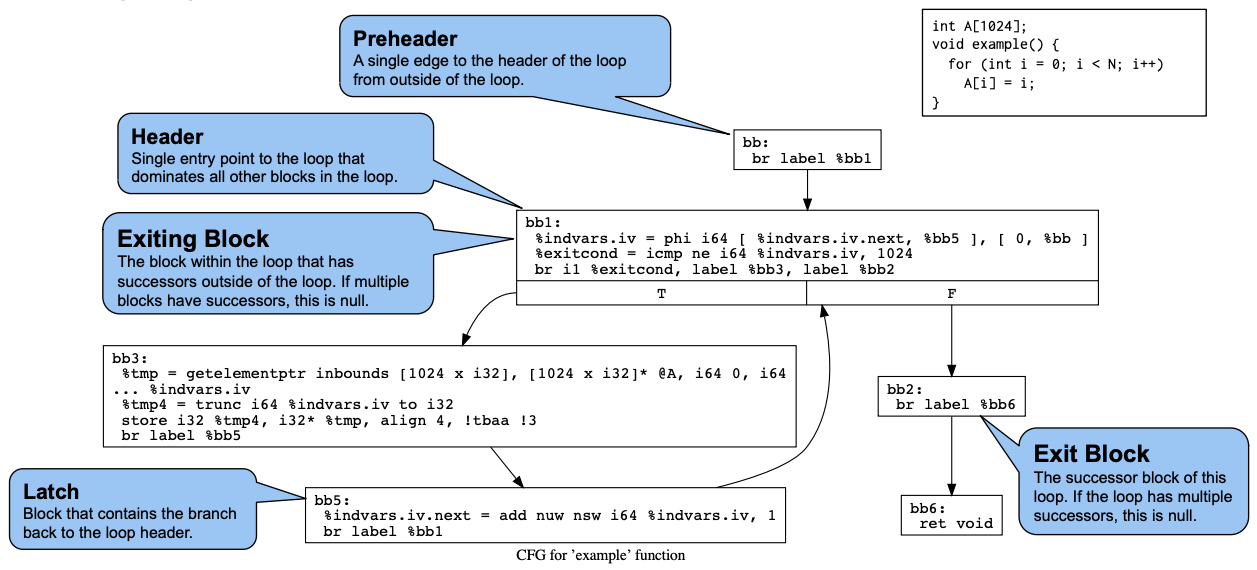
\includegraphics[width=\textwidth]{figures/LoopRepresentation.png}
\end{frame}



\begin{frame}[label=loopnormalform,fragile]{Canonical Loop Form} %MK
\framesubtitle{MK: Feel free to re-use/eliminate this slide; maybe it's useful}
\begin{columns}
\begin{column}{0.6\textwidth}
\begin{itemize}
\item Loop identified by header
\item Preheader
\item Single backedge/latch
\item Exits only from loop
\item Loop-rotated form\\(at least one iteration / loop guard)
    \begin{itemize}
    \item Can hoist invariant loads
    \end{itemize}
\item Loop-Closed SSA

%\item Responsible passes
%\begin{itemize}
%\item LoopRotate
%\item LoopSimplify
%\item IndVarSimplify
%\item LCSSA
%\end{itemize}
\end{itemize}


\end{column}
\begin{column}{0.4\textwidth}
\begin{tightcenter}
\begin{scaleenv}{0.7}
\begin{tikzpicture}
\tikzset{tight/.style={inner sep=0pt,outer sep=0pt,minimum size=0pt}}
\tikzset{invisible/.style={draw=none,fill=none,text=white}}

\tikzset{node/.style={line width=1.2pt,rounded corners,bottom color=white,shading angle=15,drop shadow}}
\tikzset{bb/.style={node,draw=teal,top color=teal!50}}

\graph [layered layout,edges={->},sibling distance=2cm,level distance=12mm]{
    enter1[as={}];
    enter2[as={}];
    guard[bb,as={Guard}];
    preheader[bb,as={Preheader}];
    header[bb,as={Header}];
    exiting[bb,as={Exiting}];
    exit[bb,as={Exit}];
    merge[bb,as={\phantom{MMM}}];
    latch[bb,as={Latch}];
    afterexit[as={}];
    
    {enter1,enter2}->guard;
    guard->preheader;
    guard->merge;
    preheader->header;  
    header->exiting;
    exiting->exit;
%    exiting->latch;
    latch->[thick,out=90,in=180]header;
    exit->merge;
    merge->afterexit;
    
    {[edge={draw=none}]
      header->latch,
      latch->exiting
    };
};

\path (latch) edge[draw=none,decorate,decoration={text along path,text={Backedge}},out=90,in=180] (header);
\path (exiting) edge[->,in=270,out=180] (latch);
\end{tikzpicture}
\end{scaleenv}
\end{tightcenter}
\end{column}
\end{columns}
\end{frame}


\begin{frame}[label={sec:orgac3eb21}]{Other Terminology}
  \begin{block}{}
    \begin{itemize}
    \item Loop predecessor
    \item Backedge taken count
    \item Iteration count
    \item Loop guard
    \item irreducible loops (not covered)
    \item Others?
    \end{itemize}
  \end{block}
\end{frame}

\begin{frame}[label={sec:rotated}]{Rotated Loops}
  \begin{itemize}
    \item Describe what rotated loops are
    \item Give some examples of rotated loops
    \item Limitations of loop rotation
  \end{itemize}
\end{frame}

\begin{frame}[label={sec:canonical}]{Canonical Form}
Describe loop canonical form - what exactly this entails, \textit{etc}.
\end{frame}


\begin{frame}[fragile,label={sec:lcssa}]{Loop-Closed SSA Form}
%    What exactly is this? When is it useful? What are the implications afterwards?

\begin{tikzpicture}
\tikzset{indent/.style={xshift=5mm}}]
\tikzset{lcssa/.style={subgraph text none,bottom color=teal!30,top color=teal!15,shading angle=15,rounded corners,draw=teal,very thick}}
\tikzset{ssa/.style={subgraph text none,bottom color=red!30,top color=red!15,shading angle=15,rounded corners,draw=red,very thick}}

\matrix[matrix of nodes,nodes={anchor=west,inner ysep=0.4ex}] {
                      \llvminline{loop:}                                                       \\
|(indvar) [indent]|     \llvminline{%indvar = phi i64 [%indvar.next, %loop], [0, %preheader]}  \\[1.5ex]
|(sum) [indent]|        \llvminline{%sum = phi i64 [%sum.next, %loop], [0, %preheader]}        \\
|(sumnext) [indent]|    \llvminline{%sum.next = add i64 %sum, %indvar}                         \\[1.5ex]
|(indvarnext) [indent]| \llvminline{%indvar.next = add i64 %indvar, 1}                         \\
|(cond) [indent]|       \llvminline{%cond = icmp ne i64 %indvar.next, 64}                      \\
|(br) [indent]|         \llvminline{br i1 %cond, label %loop, label %exit}                     \\[1.5ex]
 
                     \llvminline{exit:}        \\
|(sumresult) [indent,visible on=<2->]| \llvminline{%sum.result = phi i64 [%sum.next, %loop]}        \\[3ex]
\node[anchor=west,inner ysep=0.4ex,indent](dots1){\dots};
\node[right=0pt of dots1](use){\texttt{\alt<1>{\%sum.next}{\%sum.result}}}; 
\node[right=0pt of use]{\dots};  \\
};

\begin{pgfonlayer}{background}
\node[fit={(sum) (sumnext)},ssa] {};
\node<1>[fit={(use)},ssa] {};
\node<2->[fit={(sumresult)},lcssa] {};
\node<2->[fit={(use)},lcssa] {};
\end{pgfonlayer}
\end{tikzpicture}%
\begin{locate}<only@3->[anchor=center]{page cs:x=0.5,y=0.5}
\begin{minipage}{0.75\textwidth}
\begin{block}{}
\begin{itemize}
\item Added by LCSSA pass
    \begin{itemize}
    \item Automatically added by LoopPassManager
    \end{itemize}
\item Must be preserved by loop passes
    \begin{itemize}
    \item Helper: \cppinline{llvm::formLCSSA(Loop &L, ...)}
    \end{itemize}
\item Removed again by InstCombine
\end{itemize}
\end{block}
\bigskip
\begin{block}{Advantages}
\begin{itemize}
\item Loop transformations change only the LCSSA node
\item No need to pass scope to ScalarEvolution 
\end{itemize}
\end{block}
\end{minipage}
\end{locate}
\end{frame}






%MK: Not sure whether I am going to need this; for now it's for testing whether tikzpictruew works
\begin{frame}[fragile]{Clang/LLVM/Polly Compiler Pipeline} %MK
\begin{resizepar}
\begin{tikzpicture}
\tikzset{tight/.style={inner sep=0pt,outer sep=0pt,minimum size=0pt}}
\tikzset{node/.style={draw=teal,line width=1.2pt,rounded corners,top color=teal!50,bottom color=white,shading angle=15,drop shadow}}
\tikzset{supernode/.style={subgraph text none,bottom color=teal!30,top color=teal!05,shading angle=15,rounded corners}}
\tikzset{edge/.style={->}}

\graph[layered layout,edges={edge,rounded corners},level sep=5mm,sibling sep=10mm]{
	c[as={\minibox{\texttt{void f() \{}\\\hspace*{4mm}\texttt{for (int i=...)}\\\hspace*{4mm}\dots}},grow=right,draw,shape=file,fill=white,label={source.c}];
	ir[as={IR},shape=file,draw,fill=white,nudge=(up:10mm)];
	asm[as={Assembly},shape=file,draw,fill=white];

	clang [subgraph text none,label={[font=\Large\sffamily]above:Clang}] // [sibling sep=2mm,grow=down,layered layout] {
		lexer [as={Lexer},node];
		parser [as={Parser},node,grow=down];
		preprocessor [as={Preprocessor},node];
		sema [as={Semantic Analyzer},node];
		codegen [as={IR Generation},node];
		%
		lexer->preprocessor->parser->sema->codegen;
	};

	llvm [subgraph text none,label={[font=\Large\sffamily]above:LLVM}] // [sibling sep=2mm,grow=down,layered layout] {
		canonicalization [as={Canonicalization passes},node];
		loopopts [as={Loop optimization passes},node];
		polly [as={Polly},node];
		vectorization [as={LoopVectorize},node];
		latepasses [as={Late Mid-End passes},node];
		backend [as={Target Backend},node];
		%
		canonicalization->loopopts->vectorization->latepasses->backend;
		loopopts->polly->vectorization;
	};

	c->[in=180]lexer;
	codegen->[out=0,in=-90]ir;
	ir->[out=90,in=180]canonicalization;
	backend->[out=0,in=-90]asm;
};

\begin{pgfonlayer}{background}
\node[tight,fit={(clang)},supernode]{};
\node[tight,fit={(llvm)},supernode]{};
\end{pgfonlayer}

%	\path (preprocessor) edge[edge,densely dotted,bend left=50,draw=blue!50!black] node[midway,right,font=\ttfamily,blue!50!black] {\#pragma} (sema);
%	\path (preprocessor) edge[edge,densely dotted,bend right=80,draw=blue!50!black] node[pos=0.7,left,font=\ttfamily,blue!50!black] {\#pragma} (codegen);

	\path (codegen) edge[edge,dashed,bend right=80,draw=blue!50!black,postaction={decorate,decoration={text along path,text={|\color{blue!50!black}|Loop metadata},raise=-1.7ex,pre=moveto,pre length=13mm}}] (ir);
	\path (ir) edge[edge,dashed,draw=blue!50!black] (loopopts);
%	\path (ir) edge[edge,dashed,draw=blue!50!black] (polly);1
	\path (ir) edge[edge,dashed,draw=blue!50!black,bend right=10] (vectorization);
%	\path (polly) edge[edge,dashed,draw=blue!50!black,bend right=10] (vectorization);
\end{tikzpicture}
\end{resizepar}
\end{frame}


\begin{frame}[fragile,shrink=10]{Loop Transformation Passes} %MK
%\begin{itemize}
%\item Transformation passes:
\begin{columns}
\begin{column}[t]{0.45\textwidth}
\makeatletter
\patchcmd{\@listI}{\itemsep3\p@}{\itemsep0em}{}{}
\makeatother
\begin{itemize}
\item LoopSinkPass
\item LoopDataPrefech
\item LoopLoadElimination
\item LoopFuse
\item LoopDistribution
\item LoopVectorize
\item LoopInvariantCodeMotion (LICM)
\item VersioningLICM
\item LoopIdiomRecognize
\item LoopDeletion
\item LoopExtractor
\item Polly
\end{itemize}
\end{column}

\begin{column}[t]{0.5\textwidth}
\makeatletter
\patchcmd{\@listI}{\itemsep3\p@}{\itemsep0em}{}{}
\makeatother
\begin{itemize}
\item LoopReroll
\item LoopStrengthReduction
\item InductiveRangeCheckElimination (IRCE)
\item LoopUnrollAndJam
\item Loop(Full/Partial)Unroll
\item LoopPredication
\item GuardWidening
\item (Simple)LoopUnswitch
\item LoopInterchange
\item MachinePipeliner/SwingSchedulerDAG
\item LoopDataPrefetch
\item StructurizeCFG 
\item WebAssemblyFixIrreducibleControlFlow
\end{itemize}
\end{column}
\end{columns}
\end{frame}


\begin{frame}{Available Infrastructure} %MK
\begin{columns}
\begin{column}[t]{0.45\textwidth}
\begin{itemize}
\item Analysis passes
\begin{itemize}
\item LoopInfo
\item MemoryDependenceAnalysis
\item LoopAccessAnalysis
\item (Predicated)ScalarEvolution
\item PolyhedralInfo
\item DivergenceAnalysis
\item BlockFrequencyInfo
\end{itemize}
\end{itemize}
\end{column}


\begin{column}[t]{0.45\textwidth}
\begin{itemize}
\item Canonicalization passes
\begin{itemize}
\item LoopSimplify
\item LoopRotate
\item LoopSimplifyCFG
\item LoopClosedSSA (LCSSA)
\item IndVarSimplify
\end{itemize}
\end{itemize}
\end{column}
\end{columns}

\bigskip

\begin{columns}
\begin{column}[t]{0.45\textwidth}
\begin{itemize}
\item Utilities
\begin{itemize}
\item IVUsers
%\item LoopInterchangeLegality
%\item LoopInterchangeCodeModel,I
%\item LoopVectorizationCostModel
%\item UnrolledInstAnalyzer
\item LoopVersioning
\item SCEVExpander
\item OptimizationRemarkEmitter
%\iem LazyBlockFrequencyInfoPass
\item IrreducibleGraph
\end{itemize}
\end{itemize}
\end{column}



\begin{column}[t]{0.45\textwidth}
\begin{itemize}
\item Verification
\begin{itemize}
\item LCSSAVerificationPass
\end{itemize}
\end{itemize}

\end{column}
\end{columns}

\end{frame}



\begin{comment}

\newcommand\looppasspipeline{%
\begin{scalepar}{0.53}
\begin{tightcenter}
\begin{tikzpicture}
\tikzset{tight/.style={inner sep=0pt,outer sep=0pt,minimum size=0pt}}
\tikzset{looppass/.style={draw=teal,line width=1.2pt,rounded corners,top color=teal!50,bottom color=white,shading angle=15,drop shadow}}
\tikzset{nodenoop/.style={draw=teal,line width=1.2pt,rounded corners,top color=gray!50,bottom color=white,shading angle=15,drop shadow}}
\tikzset{nodedisabled/.style={draw=gray,line width=1.2pt,rounded corners,top color=gray!50,bottom color=white,shading angle=15,drop shadow,text=gray}}
\tikzset{supernode/.style={subgraph text none,bottom color=teal!30,top color=teal!05,shading angle=15,rounded corners}}
\tikzset{edge/.style={->,rounded corners}}

\graph[layered layout,edges={edge},level sep=3mm]{
  codegen[looppass,as={Clang CGOpenMPRuntime}],
  ir[as={IR},shape=file,draw,fill=white];
  LoopUnswitch[as={(Simple-)LoopUnswitch},looppass];
  LoopDeletion[looppass];
  LoopIdiom[looppass]; 
  LoopInterchange[nodedisabled]; 
  LoopFullUnroll[looppass];
  LoopReroll[nodedisabled];
  LoopVersioningLICM[nodedisabled];
  LoopDistribute[nodenoop];
  LoopVectorize[looppass];
  LoopLoadElimination[looppass]; 
  LoopUnrollAndJam[nodedisabled];
  LoopUnroll[looppass];
  backend[as={\dots}];

  codegen -> ir -> LoopUnswitch -> LoopIdiom -> LoopDeletion -> LoopInterchange -> LoopFullUnroll -> LoopReroll -> LoopVersioningLICM -> LoopDistribute -> LoopVectorize -> LoopLoadElimination -> LoopUnrollAndJam -> LoopUnroll -> backend;
};
\end{tikzpicture}
\end{tightcenter}
\end{scalepar}
}



\newcommand\looppassesinthepipeline{%
\begin{scalepar}{0.45}
\begin{tightcenter}
\begin{tikzpicture}
\tikzset{tight/.style={inner sep=0pt,outer sep=0pt,minimum size=0pt}}

\tikzset{scalarpass/.style={draw=none,line width=1.2pt,rounded corners,top color=gray!50,bottom color=white,shading angle=15,drop shadow}}
\tikzset{loopcanon/.style={draw=red,line width=1.2pt,rounded corners,top color=darkspringgreen!50,bottom color=white,shading angle=15,drop shadow}}
\tikzset{loopanalysis/.style={draw=none,line width=1.2pt,rounded corners,top color=teal!50,bottom color=white,shading angle=15,drop shadow}}
\tikzset{looppass/.style={draw=teal,line width=1.2pt,rounded corners,top color=teal!50,bottom color=white,shading angle=15,drop shadow}}

\tikzset{edge/.style={->,rounded corners}}

% -loops -loop-simplify -lcssa-verification -lcssa -basicaa -aa -scalar-evolution -loop-rotate -licm -loop-unswitch -simplifycfg -domtree -basicaa -aa -loops -lazy-branch-prob -lazy-block-freq -opt-remark-emitter -instcombine -loop-simplify -lcssa-verification -lcssa -scalar-evolution -indvars -loop-idiom -loop-deletion
\graph[layered layout,edges={edge},level sep=-1mm]{
  ir[as={\dots},tight];
  SimplifyCFG1[scalarpass,as={SimplifyCFG}];
  Reassociate[scalarpass];
  LoopInfo1[loopanalysis,as={LoopInfo}];
  LoopSimplify1[loopcanon,as={LoopSimplify}];
  LCSSA1[loopcanon,as={LCSSA}];
  LoopRotate[loopcanon];
  LICM[scalarpass];
  LoopUnswitch[looppass];
  SimplifyCFG2[scalarpass,as={SimplifyCFG}];
  LoopInfo2[loopanalysis,as={LoopInfo}];
  InstCombine[scalarpass];
  LoopSimplify2[loopcanon,as={LoopSimplify}];
  LCSSA2[loopcanon,as={LCSSA}];
  IndVarSimplify[loopcanon];
  LoopIdiom[looppass];
  LoopDeletion[looppass];
  dots[as={\dots}];

  ir -> SimplifyCFG1 -> Reassociate ->  LoopInfo1 -> LoopSimplify1 -> LCSSA1 -> LoopRotate -> LICM -> LoopUnswitch -> SimplifyCFG2 -> LoopInfo2 -> InstCombine -> LoopSimplify2 -> LCSSA2 ->  IndVarSimplify -> LoopIdiom -> LoopDeletion -> dots;
};
\end{tikzpicture}
\end{tightcenter}
\end{scalepar}
}



\begin{frame}[fragile]{Static Loop Pipeline} %MK
\begin{columns}
\begin{column}{0.15\textwidth}
\looppasspipeline
\end{column}
\begin{column}{0.85\textwidth}
\begin{itemize}
\item Fixed transformation order
    \begin{itemize}
    \item OpenMP outlining happens first
        \begin{itemize}
        \item Difficult to optimize afterwards
        \end{itemize}
    \item May conflict with source directives:
    \begin{minted}{c}
    #pragma distribute
    #pragma interchange
    for (int i = 1; i < n; i+=1)
      for (int j = 0; j < m; j+=1) {
        A[i][j] = i + j;
        B[i][j] = A[i-1][j];
      }
    \end{minted}
    \item OpenMP proposal: \url{https://arxiv.org/abs/1805.03374}
    \end{itemize}
\end{itemize}
\end{column}
\end{columns}
\end{frame}



\begin{frame}{Non-Loop Passes Between Loop Passes} %MK
\begin{columns}
\begin{column}{0.1\textwidth}
\looppassesinthepipeline
\end{column}
\begin{column}{0.9\textwidth}
\begin{itemize}
\item Non-loop passes may destroy canonical loop structure
\begin{itemize}
\item SimplifyCFG removes empty loop (pre-)headers
    \begin{itemize}
    \item Keeps a list of loop headers
    \item LoopSimplifyCFG only merges blocks within loop
    \item Fixed in r343816
    \end{itemize}
\item JumpThreading skips exiting block
    \begin{itemize}
    \item Has an integrated loop header detection
    \item Makes ScalarEvolution not recognize the loop
    \item Fixed in r312664(?)
    \end{itemize}
\item Bit-operations created by InstCombine must be understood by ScalarEvolution
\item LCSSA removed
\end{itemize}

\item Analysis invalidation / Extra work in non-loop passes
\end{itemize}
\end{column}
\end{columns}
\end{frame}
\end{comment}




\begin{frame}[label={sec:auxdatastruct}]{Auxiliary Data Structures}
    \begin{itemize}
    \item Dominator/PostDominator trees
    \item Data dependence graph (DDG)
    \item Others??
    \end{itemize}
\end{frame}

\section{Considerations when writing a loop pass}
\begin{frame}[label={sec:looppass}]{Loop Pass vs Function Pass}
  \begin{itemize}
  \item What is a loop pass
  \item What is a function pass
  \item Differences/pros/cons of using one over the other
  \end{itemize}
\end{frame}

\begin{frame}[label={sec:passmanager}]{Pass Managers}
  \begin{itemize}
    \item New Pass Manager
    \item Legacy Pass Manager (JD: I would only mention: use the new one)
    \item Where to put loop optimizations in the loop opt pipeline (maybe on new slide)
  \end{itemize}
\end{frame}


\section{Simple Loop Optimization Pass}
\begin{frame}[label=step1]{Basic Loop Optimization Pass using New Pass
    Manager}{\textbf{Kit to do}}
\end{frame}

\begin{frame}[label=step2]{Checking For Valid Candidates}{\textbf{Kit to do}}
\end{frame}

\begin{frame}[label=step3]{Splitting a loop using cloning}{\textbf{Ettore to do}}
\end{frame}

\begin{frame}[label=step4]{Updating data structures - dominator tree and
    SCEV}{\textbf{Kit to do}}
\end{frame}

\begin{frame}[label=step5]{Reporting Success and failure}{\textbf{Ettore to do}}
\end{frame}

\section{Other Useful Tools}
\begin{frame}[label=reports]{Reporting success and failure}
  \begin{itemize}
    \item STATISTICS
    \item Optimization Remark Emitter
  \end{itemize}
\end{frame}

\begin{frame}[label={sec:datastructs}]{Updating Data Structures}
    \begin{itemize}
      \item DominatorTreeUpdater
      \item SCEV
      \item Other??
    \end{itemize}
\end{frame}

\section{Dependence Graphs}
\begin{frame}[label={sec:DepGraphs}]{Dependence Graphs}
  \begin{itemize}
    \item Represents data dependencies between program elements (instructions)
    \item Ideas: 
    \begin{itemize}
      \item D.J. Kuck, R.H. Kuhn, D.A. Padua, B. Leasure, and M. Wolfe (1981). Deendence Graphs and Compiler Optimizations. 
      \item J. Ferrante, K.J. Ottenstein and Joe D. Warren (1987). The Program Dependence Graph and Its Use in Optimizations.
    \end{itemize}
    \item Data Dependence Graph (DDG): hierarchical representation, nodes that are part of an SCC grouped into pi-blocks
    \item Program Dependence Graph (PDG): capable of representing both data dependencies and control-flow dependencies
  \end{itemize}
\end{frame}

\begin{frame}[label=DDGExample1]{Data Dependence Graph Example}
  \begin{itemize}
    \item Example code contains a statement that has a loop carried data dependence on itself
    \item Instructions (nodes) are connected by edges to represent dependencies (def-use and memory)
    \item Def-use relations and a memory access dependency form a cycle representing the loop carried dependence.
  \end{itemize}
  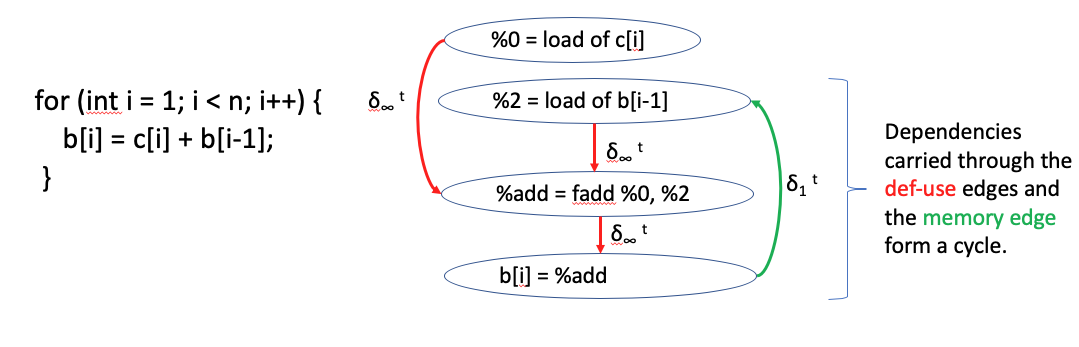
\includegraphics[width=\textwidth]{figures/DDG1.png}
\end{frame}

\begin{frame}[label=DDGExample2]{Data Dependence Graphs Example}
  \begin{itemize}
    \item The DDG corresponding to the example contains a pi-block 
    \item The pi-block groups the nodes that participate in the dependency cycle.
    \item The resulting graph is acyclic.
  \end{itemize}
  \begin{figure}[h]
  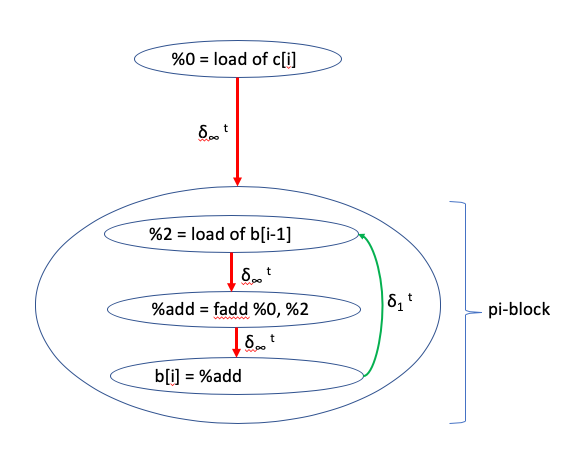
\includegraphics[width=0.55\textwidth]{figures/cycle_pi.png}
  \end{figure}
\end{frame}

\begin{frame}[label=DDGLLVM]{Data Dependence Graphs in LLVM}
  \begin{itemize}
  \item Directed Graph: D64088 (base class for various dependence graphs)
  \item Data Dependence Graph (DDG): D65350 (basic framework), D67970 (root-node), ...  
  \item Program Dependence Graph (PDG): will follow after DDG (leverage common graph builder)
  \item Envisioned Consumers:
    \begin{itemize}
    \item Loop Fusion
    \item Loop Fission
    \end{itemize}
  \end{itemize}
\end{frame}

\end{document}
